\documentclass[oneside,12pt,letterpaper]{article}

\usepackage{algpseudocode}
\usepackage{amsmath}
\usepackage{amsfonts}
\usepackage{amssymb}
\usepackage{amsthm}
\usepackage{arydshln}
\usepackage{fancyhdr}
\usepackage[margin=1in]{geometry}
\usepackage{graphicx}
\usepackage{listings}
\usepackage{setspace}
\usepackage{textcomp}
\usepackage{url}
\usepackage{xspace,color}

\newcommand{\hmwkTitle}{Assignment 1}
\newcommand{\hmwkDueDate}{September 10, 2020}
\newcommand{\hmwkSchool}{IUPUI}
\newcommand{\hmwkClass}{STAT 52400}
\newcommand{\hmwkClassInstructor}{Dr. Fang Li}
\newcommand{\hmwkAuthorName}{Ross Grinvalds}
% \newcommand{\E}{\mathrm{E}}
% \newcommand{\Var}{\mathrm{Var}}
% \newcommand{\Cov}{\mathrm{Cov}}
% \newcommand{\Bias}{\mathrm{Bias}}
\newcommand\m[1]{\begin{bmatrix}#1\end{bmatrix}} 
\newcommand\p[1]{\begin{pmatrix}#1\end{pmatrix}} 
\newcommand{\ri}[1]{\lstinline{#1}}  %% Short for 'R inline'

\pagestyle{fancy}
\setlength{\headheight}{15pt}
\lhead{\hmwkAuthorName}
\chead{\hmwkSchool\ \hmwkClass:\ \hmwkTitle}
\rhead{\hmwkClassInstructor}
\cfoot{\thepage}
\lstnewenvironment{rc}[1][]{
	\lstset{commentstyle=\color{red}, keywordstyle=\color{black}, showstringspaces=true, language=R, basicstyle=\ttfamily\tiny}
}{}
\lstset{language=R}


\begin{document}
	\title{
			\vspace{1in}
			\textmd{\textbf{\hmwkSchool\ \hmwkClass:\ \hmwkTitle}}\\
			\normalsize\vspace{0.1in}\small{Due\ on\ \hmwkDueDate\ at 11:59 PM}\\
			\vspace{6in}
	}
	\author{\hmwkAuthorName}
	\date{}
	\maketitle

	\pagebreak
	\begin{enumerate}
		\item[\textbf{2.7}]
			Given A=
			$\begin{bmatrix}
				9 & -2 \\
				-2 & 6 \\
			\end{bmatrix}$

			\begin{enumerate}
				\item[\textbf{a.}]
					Obtain the eigenvectors via $A\vec{v}-\lambda\vec{v}=\vec{0}$. Assume $\vec{v}\neq\vec{0}$. Then the eigenvalues of A are found by:
					\begin{align*}
						det(A - \lambda I) &= 0 \\
						det\begin{pmatrix} 9 - \lambda & -2 \\ -2 & 6 - \lambda \end{pmatrix} &= 0 \\
						\lambda^2 - 15\lambda + 50 &= 0 \\
						\lambda &= \frac{15 \pm 5}{2} \\
						\therefore \lambda_{1} = 10,\ \lambda_{2} = 5 \\
					\end{align*}
					
					For $\lambda_{1}$:
					\begin{align*}
						\begin{bmatrix} 9 & -2 \\ -2 & 6 \\ \end{bmatrix} \begin{bmatrix}	v_{1} \\ v_{2} \\\end{bmatrix} & =10 \begin{bmatrix}v_{1} \\ v_{2} \end{bmatrix} \\
						\implies 9 v_{1} -2 v_{2} &= 10 v_{1}
					\end{align*}
					
					Let $v_{2} = 1$, then $v_{1} = -2$. Normalizing the vector yields: $$e_{1} = \begin{pmatrix} \frac{-2 \sqrt{5}}{5} \\ \frac{\sqrt{5}}{5} \end{pmatrix}$$ Similarly, for $\lambda_{2}$:
					\begin{align*}
						\begin{bmatrix} 9 & -2 \\ -2 & 6 \\ \end{bmatrix} \begin{bmatrix}	v_{1} \\ v_{2} \\\end{bmatrix} &= 5 \begin{bmatrix}v_{1} \\ v_{2} \end{bmatrix} \\
						\implies 9 v_{1} -2 v_{2} &= 5 v_{1}
					\end{align*}

				Let $v_{1}=1$, then $v_{2}=2$. Therefore: $$e_{2} = \begin{pmatrix} \frac{\sqrt{5}}{5} \\ \frac{2 \sqrt{5}}{5} \end{pmatrix}$$
			
				\item[\textbf{b.}]
					The spectral decomposition of $A$ is:
					\begin{align*}
					A &= \lambda_{1} \vec{e_{1}} \vec{e_{1}}^\intercal + \lambda_{2} \vec{e_{2}} \vec{e_{2}}^\intercal \\
					  &= 10 \begin{bmatrix} \frac{4}{5} & -\frac{2}{5} \\ -\frac{2}{5} & \frac{1}{5} \end{bmatrix} + 5 \begin{bmatrix} \frac{1}{5} & \frac{2}{5} \\ \frac{2}{5} & \frac{4}{5} \end{bmatrix}
					\end{align*}

				\item[\textbf{c.}]
					The inverse matrix is obtained by: 
					\begin{align*}
						A^{-1} &= \frac{1}{det(A)} adjoint(A) \\
									 &= \frac{1}{5 \cdot 10} \begin{bmatrix} 6 & 2 \\ 2 & 9 \end{bmatrix}
					\end{align*}

				\item[\textbf{d.}]
					The eigenvalues of the inverse matrix are obtained directly:
					\begin{align*}
						A^{-1}\vec{v} &= \lambda \vec{v} \\
						AA^{-1}\vec{v} &= \lambda A \vec{v} \\
						I \vec{v} &= \lambda A \vec{v} \\
						\implies A \vec{v} &= \frac{1}{\lambda} \vec{v} \\
						\therefore \lambda_{1}=\frac{1}{5},\ \lambda_{2}=\frac{1}{10}
					\end{align*}

					The eigenvectors are obtained as performed in step \textbf{a.}. However, the eigenvectors are invariant after the transformation. Note that because the eigenvalues of the inverse matrix are the reciprocals of the eigenvalues of $A$, the order of magnitude is also reversed. Therefore, the order of the eigenvectors is reversed: $$e_{1} = \begin{pmatrix} \frac{\sqrt{5}}{5} \\ \frac{2 \sqrt{5}}{5} \end{pmatrix},\ e_{2} = \begin{pmatrix} -\frac{2 \sqrt{5}}{5} \\ \frac{\sqrt{5}}{5} \end{pmatrix}$$

				\item[\textbf{e.}]
					The square root matrix, $A^{\frac{1}{2}}$, is defined via the spectral decomposition of $A$. Let $P$ represent the matrix whose columns are the eigenvectors of $A$, and let $\Lambda$ represent a diagonal matrix whose diagonal entries are the nonincreasing set of eigenvalues of $A$. Then $A$ may be factored as: $$A = P \Lambda P^\intercal$$ This decomposition allows for simple computation of power functions on $A$:
					\begin{align*}
						A^{\frac{1}{2}} &= P \Lambda^{\frac{1}{2}} P^{\intercal} \\
														&= P \begin{bmatrix} \sqrt{\lambda_{1}} & 0 \\ 0 & \sqrt{\lambda_{2}} \end{bmatrix} P^{\intercal} \\
														&= \begin{bmatrix} -\frac{2\sqrt{5}}{5} & \frac{\sqrt{5}}{5} \\ \frac{\sqrt{5}}{5} & \frac{2 \sqrt{5}}{5} \end{bmatrix} 
						\begin{bmatrix}  \sqrt{10} & 0 \\ 0 & \sqrt{5} \end{bmatrix} 
						\begin{bmatrix}  -\frac{2\sqrt{5}}{5} & \frac{\sqrt{5}}{5} \\ \frac{\sqrt{5}}{5} & \frac{2 \sqrt{5}}{5} \end{bmatrix}
					\end{align*}

				\item[\textbf{f.}]
					From part \textbf{e.}, the eigenvalues are $\lambda(A^{\frac{1}{2}}) = \begin{bmatrix} \lambda(A) \end{bmatrix}^{\frac{1}{2}}$. Because the power non-negative, the eigenvectors remain invariant.

			\end{enumerate}
		
		\pagebreak
		\item[\textbf{2.21}]
			The singular value decomposition of a matrix provides a matrix factorization that can be used for rectangular matrices. The decomposition is similar to the spectral decomposition but utilizes left and right matrices that are the outer matrix products (square matrices) whose dimensions are, respectively, the row dimension, $n$, and the column dimension, $p$. The factorization is denoted by: $$A = U \Lambda V^\intercal$$ In this case, $U$ represents the matrix whose columns are the eigenvectors of $AA^\intercal$ and $V$ represents the matrix of eigenvectors of $A^\intercal A$.
			
			\begin{enumerate}
				\item[\textbf{a.}]
					\begin{align*}
						A^\intercal A &= 
						\begin{bmatrix}
							1 & 2 & 2 \\
							1 & -2 & 2
						\end{bmatrix}
						\begin{bmatrix}
							1 & 1 \\
							2 & -2 \\
							2 & 2
						\end{bmatrix} \\
													&=
													\begin{bmatrix}
														9 & 1 \\
														1 & 9
													\end{bmatrix}
					\end{align*}
					
					Let the eigenvalues of $A^{\intercal} A$ be denoted by $\gamma$. Because the square matrix is obtained by the quadratic expansion of $A$, the eigenvalues are the squared eigenvalues of $A$, or $\gamma = \lambda^{2}$. Obtain the eigenvalues as in $\textbf{2.7}$.
					\begin{align*}
						det \begin{pmatrix} A^{\intercal} A - \gamma I \end{pmatrix} &= \begin{pmatrix} 9 - \lambda \end{pmatrix}^{2} - 1 \\
						&= \gamma^{2} - 18 \gamma + 80 \\
						\implies \gamma &= \frac{18 \pm \sqrt{4}}{2} \\
						\therefore \gamma_{1} = 10,\ \gamma_{2} = 8
					\end{align*}
					
					The eigenvectors are thus obtained by: 
					$$\begin{bmatrix}
						9 & 1 \\
						1 & 9
					\end{bmatrix}
					\begin{bmatrix}
						v_{1} \\
						v_{2}
					\end{bmatrix}
					= \gamma_{i} 
					\begin{bmatrix}
						v_{1} \\
						v_{2}
					\end{bmatrix}$$

					For $i=1,\ 2$. The resulting normalized eigenvectors are thus:
					$$\vec{e_{1}} =
					\begin{bmatrix}
						\frac{\sqrt{2}}{2} \\
						\frac{\sqrt{2}}{2}
					\end{bmatrix},\ 
					\vec{e_{2}} =
					\begin{bmatrix}
						\frac{\sqrt{2}}{2} \\
						-\frac{\sqrt{2}}{2}
					\end{bmatrix}$$

					The right matrix is thus $V = \begin{bmatrix} \vec{e_{1}} & \vec{e_{2}} \end{bmatrix}$

				\item[\textbf{b.}]
					\begin{align*}
						AA^\intercal &= 
						\begin{bmatrix}
							1 & 1 \\
							2 & -2 \\
							2 & 2
						\end{bmatrix}
						\begin{bmatrix}
							1 & 2 & 2 \\
							1 & -2 & 2
						\end{bmatrix} \\
													&=
													\begin{bmatrix}
														2 & 0 & 4 \\
														10 & 8 & 0 \\
														4 & 0 & 8
													\end{bmatrix}
					\end{align*}

					The eigenvalues and eigenvectors are calculated as in $\textbf{a.}$ to obtain the left matrix. The eigenvalues in this case lead to a cubic solution which would be difficult to solve. However, the rank of the matrix is not full and there should be only two non-negative eigenvalues equal to those eigenvalues calculated in $\textbf{a.}$. Therefore, $\gamma_{3} = 0$, and $\gamma_{1} = 10, \gamma_{2} = 8$ are carried forward. The first two eigenvectors, those that correspond to non-negative eigenvalues, are calculated as in $\textbf{a.}$. They are:
					$$\vec{e_{1}} =
					\begin{bmatrix}
						\frac{\sqrt{5}}{5} \\
						0 \\
						\frac{2\sqrt{5}}{5}
					\end{bmatrix},\ 
					\vec{e_{2}} =
					\begin{bmatrix}
						0 \\
						1 \\
						0
					\end{bmatrix}$$

					The third eigenvector can be obtained by utilizing the properties of the normalized eigenvectors. That is, $\vec{e_{i}}^{\intercal}\vec{e_{3}} = 0$ for $i = 1, 2$ and $\vec{e_{3}}^{\intercal}\vec{e_{3}} = 1$. This leads to the following system of equations:
					\begin{align*}
						\begin{bmatrix}
							\frac{\sqrt{5}}{5} & 0 & \frac{2 \sqrt{5}}{5} \\
							0 & 1 & 0 \\
							1 & 1 & 1 \\
						\end{bmatrix}
						\begin{bmatrix}
							e_{1} \\
							e_{2} \\
							e_{3}
						\end{bmatrix} &=
						\begin{bmatrix}
							0 \\
							0 \\
							1
						\end{bmatrix} \\
						\therefore \vec{e_{3}} = 
						\begin{bmatrix}
							- \frac{2 \sqrt{5}}{5} \\
							0 \\
							\frac{\sqrt{5}}{5}
						\end{bmatrix}
					\end{align*}
				
				\item[\textbf{c.}]
					The singular value decomposition is expressed using the left and right matrices obtained in parts $\textbf{a.}$ and $\textbf{b.}$:
					\begin{align*}
						A &= U \Lambda V^{\intercal} \\
							&= \sum_{i=1}^{3} \lambda_{i} \vec{u_{i}} \vec{v_{i}}^{\intercal} \\
							&= \sqrt{10} 
							\begin{bmatrix}
								\frac{\sqrt{5}}{5} \\
								0 \\
								\frac{2\sqrt{5}}{5}
							\end{bmatrix} 
							\begin{bmatrix}
								\frac{\sqrt{2}}{2} & \frac{\sqrt{2}}{2}
							\end{bmatrix} + \sqrt{8} 
							\begin{bmatrix}
								0 \\
								1 \\
								0
							\end{bmatrix} 
							\begin{bmatrix}
								\frac{\sqrt{2}}{2} & - \frac{\sqrt{2}}{2}
							\end{bmatrix} \\
							&= 3.162 \ldots
							\begin{bmatrix}
								0.316 \ldots & 0.316 \ldots \\
								0 & 0 \\
								0.316 \ldots & 0.316 \ldots
							\end{bmatrix} + 2.828 \ldots
							\begin{bmatrix}
								0 & 0 \\
								0.707 \ldots & -0.707 \ldots \\
								0 & 0
							\end{bmatrix} \\
							&= \begin{bmatrix}
								1 & 1 \\
								2 & -2 \\
								2 & 2
							\end{bmatrix} \\
						\end{align*}
			\end{enumerate}

		\pagebreak
		\item[\textbf{2.25}]
			Given: $$\Sigma = \m{25&-2&4\\-2&4&1\\4&1&9}$$ $\Sigma$ represents the covariance matrix of random vector $\textbf{X}$, therefore its diagonal entries represent the marginal variances of the three random variables that compose the random vector. Let $V$ represent the diagonal matrix of the marginal variances. Then the diagonal matrix of standard deviations is: $$V^{\frac{1}{2}}=\m{5&0&0\\0&2&0\\0&0&3}$$

			In order to obtain the correlation matrix of $\textbf{X}$, each entry of $\Sigma$ needs to be divided by the pairwise standard deviations that represent the respective row and column of the entry. This can be represented in matrix notation as:
			\begin{align*}
				\boldsymbol{\rho} &= V^{-\frac{1}{2}} \Sigma V^{-\frac{1}{2}} \\
													&= \m{\frac{1}{5}&0&0\\0&\frac{1}{2}&0\\0&0&\frac{1}{3}} 
													\m{25&-2&4\\-2&4&1\\4&1&9}
													\m{\frac{1}{5}&0&0\\0&\frac{1}{2}&0\\0&0&\frac{1}{3}} \\
													&= \m{1&-\frac{1}{5}&\frac{4}{15}\\-\frac{1}{5}&1&\frac{1}{6}\\\frac{4}{15}&\frac{1}{6}&1}
			\end{align*}

		\pagebreak
		\item[\textbf{2.30}]
			Given:
			$$\textbf{X}=\m{X_{1}\\X_{2}\\X_{3}\\X_{4}}
			=\left[\begin{array}{c}X_{1}\\X_{2}\\\hdashline[2pt/2pt]X_{3}\\X_{4} \end{array}\right]
			=\left[\begin{array}{c}\boldsymbol{X^{(1)}}\\\hdashline[2pt/2pt]\boldsymbol{X^{(2)}} \end{array}\right],\ 
			\boldsymbol{\mu}_{\textbf{X}} = \m{4\\3\\2\\1},\ 
			\Sigma=\m{3&0&2&2\\0&1&1&0\\2&1&9&-2\\2&0&-2&4}$$
			Let:$$A=\m{1&2}, B=\m{1&-2\\2&-1}$$ 

			\begin{enumerate}
				\item[\textbf{a.}]
					$$E[\boldsymbol{X^{(1)}}] 
					= E\m{X_{1}\\X_{2}} 
					= \m{E[X_{1}]\\E[X_{2}]} 
					= \m{4\\3}$$

				\item[\textbf{b.}]
					$$E[A\boldsymbol{X^{(1)}}] 
					= A \cdot E\m{X_{1}\\X_{2}} 
					= \m{1&2} \m{4\\3} 
					= 10$$
				
				\item[\textbf{c.}]
					$$Cov[\boldsymbol{X^{(1)}}] 
					= Cov\p{\m{X_{1}\\X_{2}}, \m{X_{1}\\X_{2}}} 
					= \Sigma_{11} 
					= \m{3&0\\0&1}$$

				\item[\textbf{d.}]
					$$Cov[A\boldsymbol{X^{(1)}}] 
					= Cov\p{A\m{X_{1}\\X_{2}}, A\m{X_{1}\\X_{2}}} 
					= A\Sigma_{11}A^{\intercal} 
					= \m{1&2} \m{3&0\\0&1} \m{1\\2}
					= 7$$
	
				\item[\textbf{e.}]
					$$E[\boldsymbol{X^{(2)}}] 
					= \m{2\\1}$$

				\item[\textbf{f.}]
					$$E[B\boldsymbol{X^{(2)}}] 
					= \m{1&-2\\2&-1} \m{2\\1} 
					= \m{0\\3}$$
	
				\item[\textbf{g.}]
					$$Cov[\boldsymbol{X^{(2)}}] 
					= Cov\p{\m{X_{3}\\X_{4}}, \m{X_{3}\\X_{4}}} 
					= \Sigma_{22} 
					= \m{9&-2\\-2&4}$$

				\item[\textbf{h.}]
					$$Cov[B\boldsymbol{X^{(2)}}] 
					= B \Sigma_{22} B^{\intercal}
					= \m{1&-2\\2&-1} \m{9&-2\\-2&4} \m{1&2\\-2&-1}
					= \m{33&36\\36&48}$$

				\item[\textbf{i.}]
					$$Cov\p{\boldsymbol{X^{(1)}},\boldsymbol{X^{(2)}}} 
					= Cov\p{\m{X_{1}\\X_{2}}, \m{X_{3}\\X_{4}}} 
					= \Sigma_{12} 
					= \m{2&2\\1&0}$$

				\item[\textbf{j.}]
					$$Cov\p{A\boldsymbol{X^{(1)}},B\boldsymbol{X^{(2)}}} 
					= A \Sigma_{12} B^{\intercal}
					= \m{1&2} \m{2&2\\1&0} \m{1&2\\-2&-1}
					= \m{0&6}$$

			\end{enumerate}

		\pagebreak
		\item[\textbf{2.38}]
			This problem focuses on the ratio of a quadratic form of $\vec{x}$ to the squared length of the random vector $\vec{x}$ when $\vec{x} \neq \vec{0}$. An example matrix is provided for a sample calculation. The ratio is defined as: $$\frac{\vec{x}^{\intercal}A\vec{x}}{\vec{x}^{\intercal}\vec{x}}$$ The example matrix for the problem is: $$A=\m{13&-4&-2\\-4&13&-2\\2&-2&10}$$ 

			If the matrix $A$ is positive definite, the problem is greatly simplified. First, assume that the matrix is positive definite. Let the matrix $P$ represent a matrix whose columns are the normalized eigenvectors of $A$ and let the transformation $\vec{y}=P^{\intercal}\vec{x}$. The ratio can be written as:
			\begin{align*}
				\frac{\vec{x}^{\intercal}A\vec{x}}{\vec{x}^{\intercal}\vec{x}} 
				&= \frac{\vec{x}^{\intercal}A^{\frac{1}{2}}A^{\frac{1}{2}}\vec{x}}{\vec{x}^{\intercal}I\vec{x}} \\
				&= \frac{\vec{x}^{\intercal}P\Lambda^{\frac{1}{2}}\Lambda^{\frac{1}{2}P^{\intercal}}\vec{x}}{\vec{x}^{\intercal}PP^{\intercal}\vec{x}} \\
				&= \frac{\vec{y}^{\intercal}\Lambda\vec{y}}{\vec{y}^{\intercal}\vec{y}} \\
				&= \frac{\sum_{i=1}^{3}\lambda_{i}y_{i}^{2}}{\sum_{i=1}^{3}y_{i}^{2}} 
				&\leq \frac{\lambda_{1}\sum_{i=1}^{3}y_{i}^{2}}{\sum_{i=1}^{3}y_{i}^{2}} = \lambda_{1}\\
				&&\geq \frac{\lambda_{3}\sum_{i=1}^{3}y_{i}^{2}}{\sum_{i=1}^{3}y_{i}^{2}} = \lambda_{3}
			\end{align*}

			This result suggests that as long as $A$ is positive definite, the optimization of quadratic forms on $\vec{x}$ is equivalent to computing the eigenvalues of $A$ and selecting the appropriate eigenvalue. The matrix was entered in R and the eigenvalues were computed as $\lambda_{1}=18,\lambda_{2}=9,\lambda_{3}=9$. Therefore, the maximum of the ratio is $18$ and the minimum is $9$.
		\pagebreak
		\item[\textbf{1.2}]
			\begin{enumerate}
				\item[\textbf{a.}]
					Data from a morning newpaper lists used-car prices for a certain foreign compact car. The variable $x_{1}$ represents age in years and $x_{2}$ the selling price in thousands of dollars. A scatter plot of the data is provided below. It is clear that there is a strong negative association between these variables. That is, as the car ages (years increase), the value of the car degrades (selling price decreases). This should be expected as most automobiles are considered as liabilities that quickly become outdated with new technology.
					\begin{center} 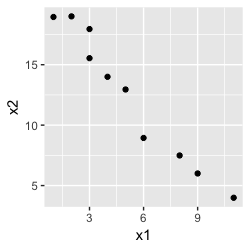
\includegraphics{plot1_2_1.png} \end{center}

				\item[\textbf{b.}]
					Because there is a negative association between $x_{1}$ and $x_{2}$, the sign of the correlation coefficient that measures the association should be negative.

				\item[\textbf{c-d.}]
					The computed sample mean vector, sample covariance matrix, and correlation matrix can be expressed as:
					$$\vec{\bar{\textbf{x}}}=\p{5.2\\12.481},
					\textbf{S}_{10}=\m{10.622&-17.710\\-17.710&30.854},
					\textbf{R}=\m{1&-0.978\\-0.978&1}$$

					The interpretation of these values is as follows. The average age of the cars in this market is $5.2$ years with an average selling price of $\$ 12,481$. The standard deviation of the age is $3.25$ years and the standard deviation of the selling price is $\$ 5,554$. The correlation coefficient confirms the extreme degree of the negative relationship between age and selling price. There is nearly a perfect negative association. 

			\end{enumerate}

		\pagebreak
		\item[\textbf{1.17-18}]
			This problem focuses on national track record data for women from 54 different countries. The first column is a categorical variable that represents the respective country. The proceeding columns represent records for increasingly longer event distances. It should be expected that record times increase as event distances increase. It is also intuitive to assume that the average speed decreases with an increasing event distance. The R output representing the sample mean vector, sample covariance matrix, and sample correlation matrix are shown below. \newline
			\begin{rc}
	> DATA %>% select(-X1) %>% summarise_all(funs(mean)) %>% as.matrix()
	  X2       X3       X4       X5       X6       X7       X8
	[1,] 11.35778 23.11852 51.98907 2.022407 4.189444 9.080741 153.6193

	> cov(DATA[,2:8])
	  X2         X3         X4          X5         X6          X7         X8
	X2 0.15531572  0.3445608  0.8912960 0.027703564 0.08389119  0.23388281   4.334178
	X3 0.34456080  0.8630883  2.1928363 0.066165898 0.20276331  0.55435017  10.384988
	X4 0.89129602  2.1928363  6.7454576 0.181807932 0.50917683  1.42681579  28.903731
	X5 0.02770356  0.0661659  0.1818079 0.007546925 0.02141457  0.06137932   1.219655
	X6 0.08389119  0.2027633  0.5091768 0.021414570 0.07418270  0.21615514   3.539837
	X7 0.23388281  0.5543502  1.4268158 0.061379315 0.21615514  0.66475793  10.706091
	X8 4.33417757 10.3849876 28.9037314 1.219654647 3.53983732 10.70609113 270.270150

	> cor(DATA[,2:8])
	  X2        X3        X4        X5        X6        X7        X8
	X2 1.0000000 0.9410886 0.8707802 0.8091758 0.7815510 0.7278784 0.6689597
	X3 0.9410886 1.0000000 0.9088096 0.8198258 0.8013282 0.7318546 0.6799537
	X4 0.8707802 0.9088096 1.0000000 0.8057904 0.7197996 0.6737991 0.6769384
	X5 0.8091758 0.8198258 0.8057904 1.0000000 0.9050509 0.8665732 0.8539900
	X6 0.7815510 0.8013282 0.7197996 0.9050509 1.0000000 0.9733801 0.7905565
	X7 0.7278784 0.7318546 0.6737991 0.8665732 0.9733801 1.0000000 0.7987302
	X8 0.6689597 0.6799537 0.6769384 0.8539900 0.7905565 0.7987302 1.0000000

			\end{rc}

			The correlations between different event distances exhibit a decay pattern which fits into the intuition mentioned above. The shorter events are much more similar than the long events. The columns $X2$ to $X8$ represent, respectively, 100 m, 200 m 400 m , 800 m, 1,500 m, 3,000 m, and 42,195 m distances. This explains why the decaying correlation is much less severe for the first several columns and more extreme for the latter. One way of imagining the decaying relationship is that the runners are exhibiting increasingly slower speeds as the distance increases. The data can be transformed to represent speeds, in meters / second, rather than times, in seconds. The updated mean vector, covariance matrix, and correlation matrix are printed below. \newline
			\begin{rc}
	> DATA.adj %>% select(-X1) %>% summarise_all(funs(mean)) %>% as.matrix()
		X2       X3       X4       X5       X6       X7       X8
	[1,] 8.814772 8.664408 7.712067 6.604214 5.989687 5.542701 4.620264

	> cov(DATA.adj[,2:8])
	  X2         X3         X4         X5         X6         X7         X8
	X2 0.09053826 0.09560635 0.09667244 0.06506402 0.08221980 0.09214221 0.08109987
	X3 0.09560635 0.11467144 0.11386990 0.07492487 0.09601895 0.10543645 0.09331033
	X4 0.09667244 0.11386990 0.13778886 0.08094090 0.09544299 0.10831645 0.10188073
	X5 0.06506402 0.07492487 0.08094090 0.07352284 0.08645423 0.09975466 0.09430563
	X6 0.08221980 0.09601895 0.09544299 0.08645423 0.12384050 0.14371481 0.11845777
	X7 0.09214221 0.10543645 0.10831645 0.09975466 0.14371481 0.17658433 0.14656043
	X8 0.08109987 0.09331033 0.10188073 0.09430563 0.11845777 0.14656043 0.16671409

	> cor(DATA.adj[,2:8])
	  X2        X3        X4        X5        X6        X7        X8
	X2 1.0000000 0.9383028 0.8655248 0.7974687 0.7764777 0.7287297 0.6601124
	X3 0.9383028 1.0000000 0.9058875 0.8159945 0.8057456 0.7409469 0.6748635
	X4 0.8655248 0.9058875 1.0000000 0.8041737 0.7306437 0.6944025 0.6722005
	X5 0.7974687 0.8159945 0.8041737 1.0000000 0.9060324 0.8754795 0.8518052
	X6 0.7764777 0.8057456 0.7306437 0.9060324 1.0000000 0.9718385 0.8244153
	X7 0.7287297 0.7409469 0.6944025 0.8754795 0.9718385 1.0000000 0.8541900
	X8 0.6601124 0.6748635 0.6722005 0.8518052 0.8244153 0.8541900 1.0000000

			\end{rc}

			The transformed data retains the correlation structure from $\textbf{1.17}$, but the covariance matrix is more interesting. Now, each of event distances exhibits highly similar variances of runner speed. This suggests that within group variation of runner speed remains stable regardless of the distance ran. This is somewhat intuitive in that the records represent world-class athletes in each event category.

		\pagebreak
		\item[\textbf{2.22}]
			This problem is similar to $\textbf{2.21}$ above. This time, the problem is completely done in R. The output showing these steps is listed below.\newline
			\begin{rc}
> # 2.22
> A = as.matrix(rbind(c(4, 8, 8), c(3, 6, -9)))
> AAt <- eigen(A %*% t(A))
> AtA <- eigen(t(A) %*% A)
> AAt$vectors[,1] %*% t(AtA$vectors[,1])
	[,1]       [,2]       [,3]
[1,] -0.16329932 -0.3265986 -0.8164966
[2,]  0.08164966  0.1632993  0.4082483
> AAt$vectors[,2] %*% t(AtA$vectors[,2])
	[,1]      [,2]       [,3]
[1,] 0.1825742 0.3651484 -0.1825742
[2,] 0.3651484 0.7302967 -0.3651484
> AAt
eigen() decomposition
$values
[1] 150 120

$vectors
	[,1]       [,2]
[1,] -0.8944272 -0.4472136
[2,]  0.4472136 -0.8944272

> AtA
eigen() decomposition
$values
[1] 1.500000e+02 1.200000e+02 2.842171e-14

$vectors
	[,1]       [,2]          [,3]
[1,] 0.1825742 -0.4082483  8.944272e-01
[2,] 0.3651484 -0.8164966 -4.472136e-01
[3,] 0.9128709  0.4082483 -7.632783e-17

> sqrt(AAt$values[1])*-1 * AAt$vectors[,1] %*% t(AtA$vectors[,1]) + 
sqrt(AAt$values[2]) * AAt$vectors[,2] %*% t(AtA$vectors[,2])
	[,1] [,2] [,3]
[1,]    4    8    8
[2,]    3    6   -9

			\end{rc}

			At the end of the output, the original matrix $A$ is recomposed from the decomposition. Again, one of the square matrices $A^{\intercal}A$ is not full rank. Notice that there is an additional eigenvalue of zero in that expansion. The non-zero eigenvalues for the two square matrices are equivalent.

	\end{enumerate}
\end{document}
